We will here make an estimate of the viscosities in the system.
We should note that this estimate is rather crude.
Following \cite{Helander2002book}, (which again is based on \cite{Braginskii1965}), we see that in a Cartesian coordinate system have that the rate of strain tensor is given by
%
\begin{align*}
    W^{ij}_{\a} \defined \partial_j u^{i}_{\a}
                     + \partial_i u^{j}_{\a}
                     - \frac{2}{3} \delta_i^j \div \ve{u}_{\a}
\end{align*}
%
which gives
% NOTE: These calculations has been double checked, and found to be OK
\begin{align*}
W^{xx} + W^{yy}
=&
\partial_x u^{x}_{\a}
+ \partial_x u^{x}_{\a}
- \frac{2}{3} \div \ve{u}_{\a}
+ \partial_y u^{y}_{\a}
+ \partial_y u^{y}_{\a}
- \frac{2}{3} \div \ve{u}_{\a}
\\
=&
2\partial_x u^{x}_{\a}
+ 2\partial_y u^{y}_{\a}
- \frac{4}{3} \div \ve{u}_{\a}
\\
=&
2\L(\partial_x u^{x}_{\a}
    + \partial_y u^{y}_{\a}
    - \frac{2}{3} \L[\partial_x u^{x}_{\a}
          +\partial_y u^{y}_{\a}
          +\partial_z u^{z}_{\a}
                      \R] \R)
\\
=&
\frac{2}{3}\L(\partial_x u^{x}_{\a}
          + \partial_y u^{y}_{\a}
          - 2\partial_z u^{z}_{\a} \R)
\\
%
%
%
W^{xx} - W^{yy}
=&
\partial_x u^{x}_{\a}
+ \partial_x u^{x}_{\a}
- \frac{2}{3} \div \ve{u}_{\a}
- \partial_y u^{y}_{\a}
- \partial_y u^{y}_{\a}
+ \frac{2}{3} \div \ve{u}_{\a}
\\
=&
2\partial_x u^{x}_{\a} -2 \partial_y u^{y}_{\a}
\\
=&
2\L(\partial_x u^{x}_{\a} - \partial_y u^{y}_{\a} \R)
\\
%
%
%
W^{zz}
=&
\partial_z u^{z}_{\a} + \partial_z u^{z}_{\a} - \frac{2}{3} \div \ve{u}_{\a}
\\
%
=&
2\partial_z u^{z}_{\a} - \frac{2}{3}
    \L(\partial_x u^{x}_{\a}
       +\partial_y u^{y}_{\a}
       +\partial_z u^{z}_{\a}
    \R)
\\
%
=&
\frac{4}{3} \partial_z u^{z}_{\a} - \frac{2}{3}
    \L(\partial_x u^{x}_{\a}
       +\partial_y u^{y}_{\a}
    \R)
\\
%
%
%
%
W^{xy}
=&
\partial_x u^{y}_{\a} + \partial_y u^{x}_{\a}
\\
%
%
%
%
W^{xz}
=&
\partial_x u^{z}_{\a} + \partial_z u^{x}_{\a}
\\
%
%
%
W^{yz}
=&
\partial_y u^{z}_{\a} + \partial_z u^{y}_{\a}
%
\end{align*}
%
We use this to calculate the components of the stress tensor.
We get
%
% NOTE: Checked that agrees with Helander
% NOTE: Checked that inserted correct
\begin{align*}
    \pi^{xx}_{\a}
    =& -\frac{\eta_{\a,0}}{2}\L(W^{xx} + W^{yy}\R)
       -\frac{\eta_{\a,1}}{2}\L(W^{xx} - W^{yy}\R)
       -\eta_{\a,3} W^{xy}
    \\
    =& -\frac{\eta_{\a,0}}{2}
            \frac{2}{3}\L(\partial_x u^{x}_{\a}
              + \partial_y u^{y}_{\a}
              - 2\partial_z u^{z}_{\a} \R)
       -\frac{\eta_{\a,1}}{2}
            2\L(\partial_x u^{x}_{\a} - \partial_y u^{y}_{\a} \R)
            -\eta_{\a,3}
       \L( \partial_x u^{y}_{\a} + \partial_y u^{x}_{\a} \R)
     \\
    =& -\frac{\eta_{\a,0}}{3}
                       \L(\partial_x u^{x}_{\a}
              + \partial_y u^{y}_{\a}
              - 2\partial_z u^{z}_{\a} \R)
       -      \eta_{\a,1}
             \L(\partial_x u^{x}_{\a} - \partial_y u^{y}_{\a} \R)
             -\eta_{\a,3}
       \L( \partial_x u^{y}_{\a} + \partial_y u^{x}_{\a} \R)
    \\
    %
    %
    %
\pi^{yy}_{\a}
    =& -\frac{\eta_{\a,0}}{2}\L(W^{xx} + W^{yy}\R)
       -\frac{\eta_{\a,1}}{2}\L(W^{yy} - W^{xx}\R)
       +\eta_{\a,3}W^{xy}
    \\
    =& -\frac{\eta_{\a,0}}{2}
    \frac{2}{3}\L(\partial_x u^{x}_{\a}
              + \partial_y u^{y}_{\a}
              - 2\partial_z u^{z}_{\a} \R)
              + \frac{ \eta_{\a,1}}{2}
       2 \L(\partial_x u^{x}_{\a} - \partial_y u^{y}_{\a} \R)
     +\eta_{\a,3}
     \L( \partial_x u^{y}_{\a} + \partial_y u^{x}_{\a} \R)
    \\
    =& -\frac{\eta_{\a,0}}{3}
                       \L(\partial_x u^{x}_{\a}
              + \partial_y u^{y}_{\a}
              - 2\partial_z u^{z}_{\a} \R)
       +      \eta_{\a,1}
             \L(\partial_x u^{x}_{\a} - \partial_y u^{y}_{\a} \R)
       +\eta_{\a,3}
       \L( \partial_x u^{y}_{\a} + \partial_y u^{x}_{\a} \R)
    \\
    %
    %
    %
\pi^{zz}_{\a}
    =& -\eta_{\a,0}W^{zz}
    \\
    =& -\eta_{\a,0}
        \L(
        \frac{4}{3} \partial_z u^{z}_{\a} - \frac{2}{3}
        \L[\partial_x u^{x}_{\a}
           +\partial_y u^{y}_{\a}
        \R]
        \R)
    \\
    =& -\frac{2\eta_{\a,0}}{3}
        \L(
        2\partial_z u^{z}_{\a} -
        \L[\partial_x u^{x}_{\a}
           +\partial_y u^{y}_{\a}
        \R]
        \R)
    \\
    %
    %
    %
\pi^{xy}_{\a} = \pi^{yx}_{\a}
=& -\eta_{\a,1} W^{xy}
    +\frac{\eta_{\a,3}}{2} \L(W^{xx}-W^{yy}\R)
    \\
    =& -\eta_{\a,1}
    \L(\partial_x u^{y}_{\a} + \partial_y u^{x}_{\a}\R)
    +\frac{\eta_{\a,3}}{2}
    2\L(\partial_x u^{x}_{\a} - \partial_y u^{y}_{\a} \R)
    \\
    =& -\eta_{\a,1}
    \L(\partial_x u^{y}_{\a} + \partial_y u^{x}_{\a}\R)
    +      \eta_{\a,3}
     \L(\partial_x u^{x}_{\a} - \partial_y u^{y}_{\a} \R)
    \\
    %
    %
    %
    %
    \pi^{xz}_{\a} = \pi^{zx}_{\a}
=& -\eta_{\a,2}W^{xz} - \eta_{\a,4}W^{yz}
    \\
    =& -\eta_{\a,2}
    \L(\partial_x u^{z}_{\a} + \partial_z u^{x}_{\a}\R)
    - \eta_{\a,4}
    \L(\partial_y u^{z}_{\a} + \partial_z u^{y}_{\a}\R)
    \\
    %
    %
    %
    \pi^{yz}_{\a} = \pi^{zy}_{\a}
    =& -\eta_{\a,2}W^{yz} + \eta_{\a,4}W^{xz}
    \\
    =& -\eta_{\a,2}
    \L(\partial_y u^{z}_{\a} + \partial_z u^{y}_{\a}\R)
    + \eta_{\a,4}
    \L(\partial_x u^{z}_{\a} + \partial_z u^{x}_{\a}\R)
\end{align*}
%
By taking the divergence of this, we find that
%
% Checked: Checked, and this agrees
\begin{align*}
    \div\te{\pi}_\a
    =&
    \ve{e}^i\cdot\partial_i \pi^{jk}_\a\ve{e}_j\ve{e}_k
    \note{Cartesian system}
    \\
    %
    =&
    \ve{e}^i\cdot\ve{e}_j\ve{e}_k\partial_i \pi^{jk}_\a
    \\
    %
    =&
    \ve{e}_k\partial_i \pi^{ik}_\a
    \\
    %
    =&
    \quad
    \ve{e}_x
    \L(
      \partial_x \pi^{xx}_\a
    + \partial_y \pi^{yx}_\a
    + \partial_z \pi^{zx}_\a
    \R)
    \\&+
    \ve{e}_y
    \L(
      \partial_x \pi^{xy}_\a
    + \partial_y \pi^{yy}_\a
    + \partial_z \pi^{zy}_\a
    \R)
    \\&+
    \ve{e}_z
    \L(
      \partial_x \pi^{xz}_\a
    + \partial_y \pi^{yz}_\a
    + \partial_z \pi^{zz}_\a
    \R)
    \\
    %
    %
    %
    =&
    \quad
    \ve{e}_x
    \L(
      \partial_x
      \L[ -\frac{\eta_{\a,0}}{3}
                       \L(\partial_x u^{x}_{\a}
              + \partial_y u^{y}_{\a}
              - 2\partial_z u^{z}_{\a} \R)
       -      \eta_{\a,1}
             \L(\partial_x u^{x}_{\a} - \partial_y u^{y}_{\a} \R)
       -\eta_{\a,3}
       \L( \partial_x u^{y}_{\a} + \partial_y u^{x}_{\a} \R)\R]
       \R.\\
       &\L.\qquad
       + \partial_y
    \L[ -\eta_{\a,1}
    \L(\partial_x u^{y}_{\a} + \partial_y u^{x}_{\a}\R)
    +      \eta_{\a,3}
     \L(\partial_x u^{x}_{\a} - \partial_y u^{y}_{\a} \R)\R]
       \R.\\
       &\L.\qquad
    + \partial_z
    \L[ -\eta_{\a,2}
    \L(\partial_x u^{z}_{\a} + \partial_z u^{x}_{\a}\R)
    - \eta_{\a,4}
    \L(\partial_y u^{z}_{\a} + \partial_z u^{y}_{\a}\R)\R]
    \R)
    %
    \\&+
    \ve{e}_y
    \L(
      \partial_x
      \L[ -\eta_{\a,1}
    \L(\partial_x u^{y}_{\a} + \partial_y u^{x}_{\a}\R)
    +      \eta_{\a,3}
     \L(\partial_x u^{x}_{\a} - \partial_y u^{y}_{\a} \R)\R]
       \R.\\
       &\L.\qquad
    + \partial_y
    \L[ -\frac{\eta_{\a,0}}{3}
                       \L(\partial_x u^{x}_{\a}
              + \partial_y u^{y}_{\a}
              - 2\partial_z u^{z}_{\a} \R)
       +      \eta_{\a,1}
             \L(\partial_x u^{x}_{\a} - \partial_y u^{y}_{\a} \R)
       +\eta_{\a,3}
       \L( \partial_x u^{y}_{\a} + \partial_y u^{x}_{\a} \R)\R]
       \R.\\
       &\L.\qquad
    + \partial_z
    \L[ -\eta_{\a,2}
    \L(\partial_y u^{z}_{\a} + \partial_z u^{y}_{\a}\R)
    + \eta_{\a,4}
    \L(\partial_x u^{z}_{\a} + \partial_z u^{x}_{\a}\R)\R]
    \R)
    %
    \\&+
    \ve{e}_z
    \L(
      \partial_x
      \L[ -\eta_{\a,2}
    \L(\partial_x u^{z}_{\a} + \partial_z u^{x}_{\a}\R)
    - \eta_{\a,4}
    \L(\partial_y u^{z}_{\a} + \partial_z u^{y}_{\a}\R)\R]
       \R.\\
       &\L.\qquad
    + \partial_y
    \L[ -\eta_{\a,2}
    \L(\partial_y u^{z}_{\a} + \partial_z u^{y}_{\a}\R)
    + \eta_{\a,4}
    \L(\partial_x u^{z}_{\a} + \partial_z u^{x}_{\a}\R)\R]
       \R.\\
       &\L.\qquad
    + \partial_z
    \L[ -\frac{2\eta_{\a,0}}{3}
        \L(
        2 \partial_z u^{z}_{\a} -
        \L[\partial_x u^{x}_{\a}
           +\partial_y u^{y}_{\a}
        \R]
        \R)\R]
    \R)
\end{align*}
%
Up until this point, we have not made any further assumptions of the $\te{\pi}$ tensor, that hasn't already been made in \cite{Braginskii1965}.
Here however, we simplify the expression (on the cost of accuracy), and say that we assume that the viscosities are constants (note that we already did such an approximation when calculating the particle flux originating from the resistivity drift when we derived $\partial_t \ln(n)$).
We then get
%
\begin{align*}
    \div\te{\pi}_\a
    \simeq&
    \quad
    \ve{e}_x
    \L(
       -\frac{\eta_{\a,0}}{3}
                       \L[\partial_x^2 u^{x}_{\a}
              + \partial_x\partial_y u^{y}_{\a}
              - 2\partial_x\partial_z u^{z}_{\a} \R]
       -      \eta_{\a,1}
             \L[\partial_x^2 u^{x}_{\a} - \partial_x\partial_y u^{y}_{\a} \R]
       -\eta_{\a,3}
       \L[ \partial_x^2 u^{y}_{\a} + \partial_x\partial_y u^{x}_{\a} \R]
       \R.\\
       &\L.\qquad
     -\eta_{\a,1}
    \L[\partial_y\partial_x u^{y}_{\a} + \partial_y^2 u^{x}_{\a}\R]
    +      \eta_{\a,3}
     \L[\partial_y\partial_x u^{x}_{\a} - \partial_y^2 u^{y}_{\a} \R]
       \R.\\
       &\L.\qquad
     -\eta_{\a,2}
    \L[\partial_z\partial_x u^{z}_{\a} + \partial_z^2 u^{x}_{\a}\R]
    - \eta_{\a,4}
    \L[\partial_z\partial_y u^{z}_{\a} + \partial_z^2 u^{y}_{\a}\R]
    \R)
    %
    \\&+
    \ve{e}_y
    \L(
      -\eta_{\a,1}
    \L[\partial_x^2 u^{y}_{\a} + \partial_x\partial_y u^{x}_{\a}\R]
    +      \eta_{\a,3}
     \L[\partial_x^2 u^{x}_{\a} - \partial_x\partial_y u^{y}_{\a} \R]
       \R.\\
       &\L.\qquad
     -\frac{\eta_{\a,0}}{3}
                       \L[\partial_y\partial_x u^{x}_{\a}
              + \partial_y^2 u^{y}_{\a}
              - 2\partial_y\partial_z u^{z}_{\a} \R]
       +      \eta_{\a,1}
             \L[\partial_y\partial_x u^{x}_{\a} - \partial_y^2 u^{y}_{\a} \R]
       +\eta_{\a,3}
       \L[ \partial_y\partial_x u^{y}_{\a} + \partial_y^2 u^{x}_{\a} \R]
       \R.\\
       &\L.\qquad
     -\eta_{\a,2}
    \L[\partial_z\partial_y u^{z}_{\a} + \partial_z^2 u^{y}_{\a}\R]
    + \eta_{\a,4}
    \L[\partial_z\partial_x u^{z}_{\a} + \partial_z^2 u^{x}_{\a}\R]
    \R)
    %
    \\&+
    \ve{e}_z
    \L(
       -\eta_{\a,2}
    \L[\partial_x^2 u^{z}_{\a} + \partial_x\partial_z u^{x}_{\a}\R]
    - \eta_{\a,4}
    \L[\partial_x\partial_y u^{z}_{\a} + \partial_x\partial_z u^{y}_{\a}\R]
       \R.\\
       &\L.\qquad
     -\eta_{\a,2}
    \L[\partial_y^2 u^{z}_{\a} + \partial_y\partial_z u^{y}_{\a}\R]
    + \eta_{\a,4}
    \L[\partial_y\partial_x u^{z}_{\a} + \partial_y\partial_z u^{x}_{\a}\R]
       \R.\\
       &\L.\qquad
       -\frac{2\eta_{\a,0}}{3}
        \L[
        2\partial_z^2 u^{z}_{\a} -
        \L(\partial_z\partial_x u^{x}_{\a}
           +\partial_z\partial_y u^{y}_{\a}
        \R)
        \R]
    \R)
    \\
    %
    %
    %
    %
    %
    =&
    \quad
    \ve{e}_x
    \L(
       -\frac{\eta_{\a,0}}{3}
                       \L[\partial_x^2 u^{x}_{\a}
              + \partial_x\partial_y u^{y}_{\a}
              - 2\partial_x\partial_z u^{z}_{\a} \R]
       -      \eta_{\a,1}
             \L[\L(\partial_x^2 + \partial_y^2\R) u^{x}_{\a} \R]
       \R.\\
       &\L.\qquad
    -      \eta_{\a,3}
     \L[\L(\partial_x^2+\partial_y^2 \R) u^{y}_{\a} \R]
       \R.\\
       &\L.\qquad
     -\eta_{\a,2}
    \L[\partial_z\partial_x u^{z}_{\a} + \partial_z^2 u^{x}_{\a}\R]
    - \eta_{\a,4}
    \L[\partial_z\partial_y u^{z}_{\a} + \partial_z^2 u^{y}_{\a}\R]
    \R)
    %
    \\&+
    \ve{e}_y
    \L(
     -\frac{\eta_{\a,0}}{3}
                       \L[\partial_y\partial_x u^{x}_{\a}
              + \partial_y^2 u^{y}_{\a}
              - 2\partial_y\partial_z u^{z}_{\a} \R]
       -      \eta_{\a,1}
        \L[\L(\partial_x^2 + \partial_y^2\R) u^{y}_{\a} \R]
       \R.\\
       &\L.\qquad
        + \eta_{\a,3}
     \L[\L(\partial_x^2 + \partial_y^2 \R)u^{x}_{\a}\R]
       \R.\\
       &\L.\qquad
     -\eta_{\a,2}
    \L[\partial_z\partial_y u^{z}_{\a} + \partial_z^2 u^{y}_{\a}\R]
    + \eta_{\a,4}
    \L[\partial_z\partial_x u^{z}_{\a} + \partial_z^2 u^{x}_{\a}\R]
    \R)
    %
    \\&+
    \ve{e}_z
    \L(
    -\frac{2\eta_{\a,0}}{3}
        \L[
        2\partial_z^2 u^{z}_{\a} -
        \L(\partial_z\partial_x u^{x}_{\a}
           +\partial_z\partial_y u^{y}_{\a}
        \R)
        \R]
       \R.\\
       &\L.\qquad
       -\eta_{\a,2}
    \L[\L(\partial_x^2  + \partial_y^2\R) u^{z}_{\a}
     + \partial_x\partial_z u^{x}_{\a}  + \partial_y\partial_z u^{y}_{\a}\R]
       \R.\\
       &\L.\qquad
    + \eta_{\a,4}
    \L[\partial_y\partial_z u^{x}_{\a}- \partial_x\partial_z u^{y}_{\a}\R]
    \R)
\end{align*}
%
We have that
%
\begin{align*}
    &\eta_{0,i}=\frac{0.96n_iT_i\sqrt{2}}{\nu_{ii}} &
    &\eta_{1,i}=\frac{3n_iT_i\nu_{ii}}{10\om_{ci}^2 \sqrt{2}} &
    &\eta_{2,i}=\frac{12n_iT_i\nu_{ii}}{10\om_{ci}^2\sqrt{2}} &
    &\eta_{3,i}=\frac{n_iT_i}{2\om_{ci}} &
    &\eta_{4,i}=\frac{n_iT_i}{\om_{ci}} &
    \\
    &\eta_{0,e}=\frac{0.73n_eT_e}{\nu_{ei}} &
    &\eta_{1,e}=0.51\frac{n_eT_e\nu_{ei}}{\om_{ce}^2} &
    &\eta_{2,e}=2.04\frac{n_eT_e\nu_{ei}}{\om_{ce}^2} &
    &\eta_{3,e}=\frac{n_eT_e}{2\om_{ce}} &
    &\eta_{4,e}=\frac{n_eT_e}{\om_{ce}} &
\end{align*}
%
and from \cref{fig:etas} we see that $\eta_{\a,0} \gg \eta_{\a,j} \quad j \in \{1,2,3,4\}$ for the parameter range that we are interested in.
Although one should look at the different terms as a whole, one could again make an approximation and say that only the terms $\propto \eta_{\a,0}$ are contributing to the viscosity tensor.
Note that this may not be a bad approximation due to the difference in magnitude for the different $\eta$s.
This would yield
%
\begin{figure}[t!]
    \centering
    \begin{subfigure}[t]{0.45\textwidth}
        \centering
        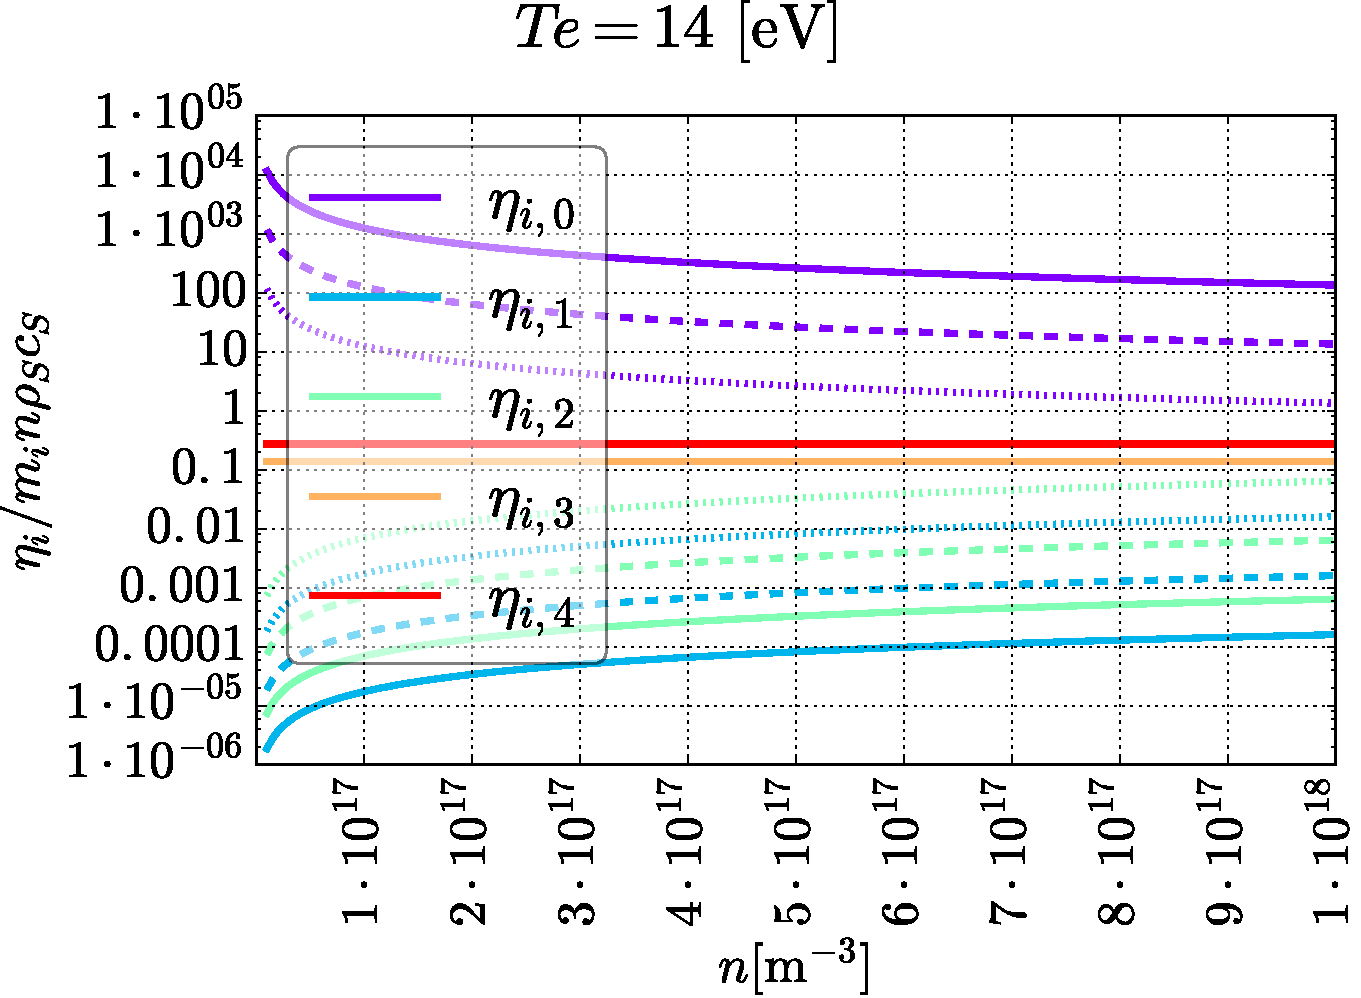
\includegraphics[width=1.0\textwidth]{fig/etaINScan}
        \caption{The normalized ion viscosities as a function of $n$}
    \end{subfigure}%
    \hfill
    \begin{subfigure}[t]{0.45\textwidth}
        \centering
        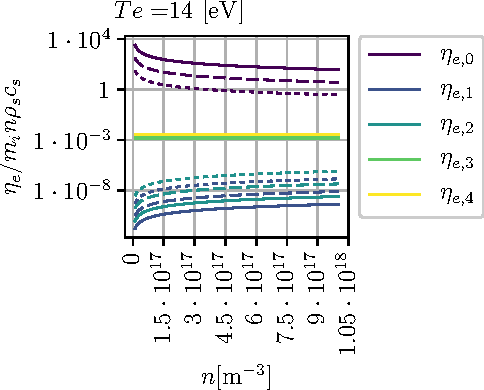
\includegraphics[width=1.0\textwidth]{fig/etaENScan}
        \caption{The normalized ion viscosities as a function of $n$}
    \end{subfigure}
    \\
    \hfill
    \begin{subfigure}[t]{0.45\textwidth}
        \centering
        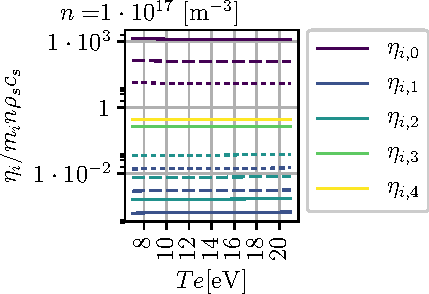
\includegraphics[width=1.0\textwidth]{fig/etaITScan}
        \caption{The normalized ion viscosities as a function of $T_e$}
    \end{subfigure}
    \hfill
    \begin{subfigure}[t]{0.45\textwidth}
        \centering
        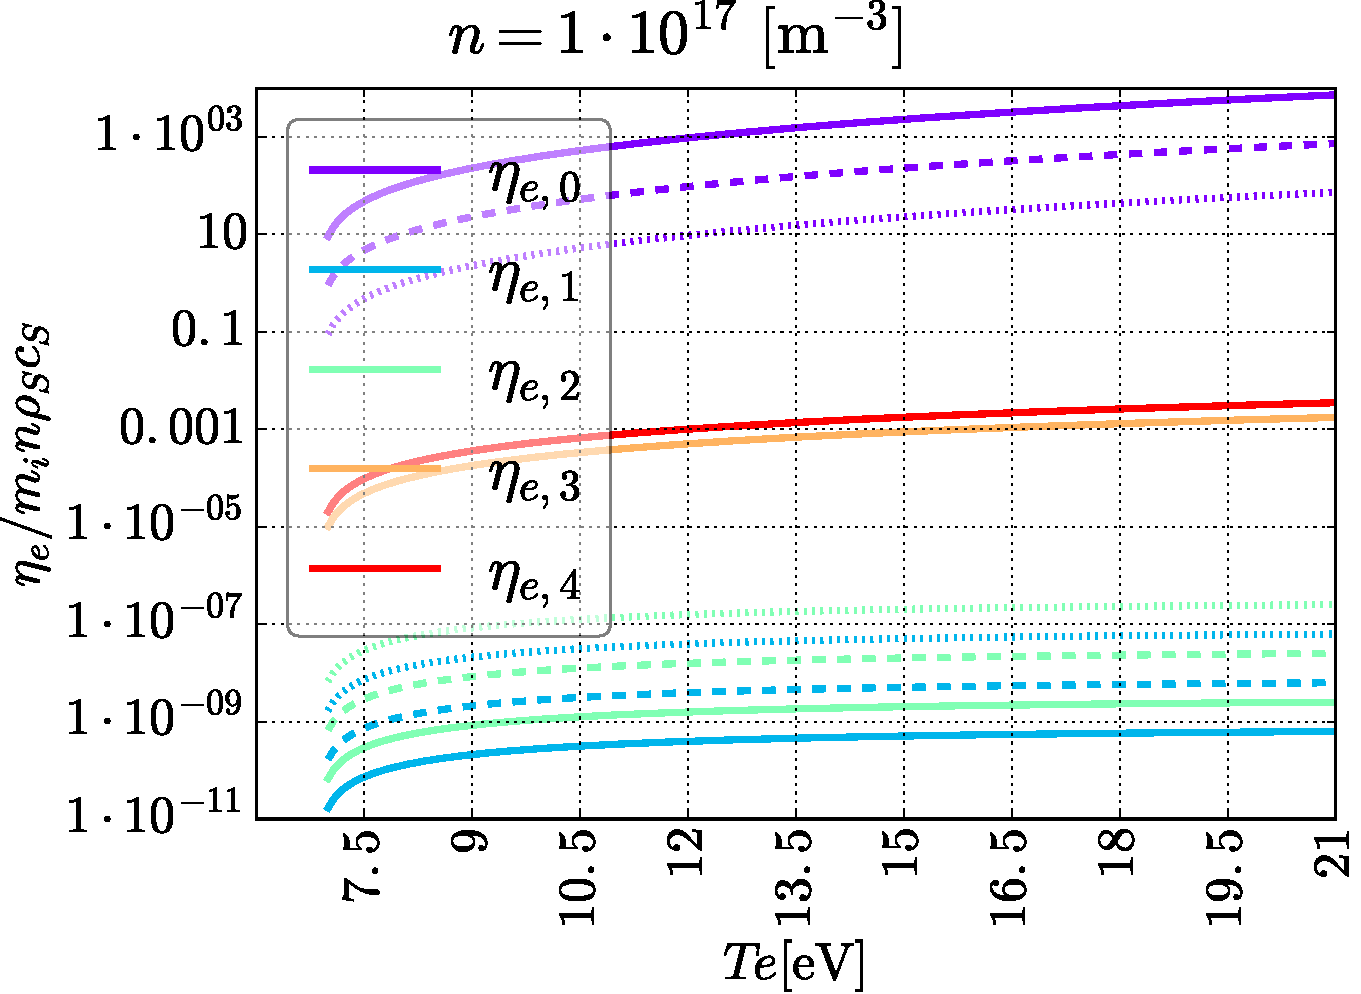
\includegraphics[width=1.0\textwidth]{fig/etaETScan}
        \caption{The normalized ion viscosities as a function of $T_e$}
    \end{subfigure}
    \caption{$\eta$ scans. The solid lines are taken at $B=1\text{ T}$, the
        dashed at $B=0.1\text{ T}$, and the dotted at $B=0.01\text{ T}$}
    \label{fig:etas}
\end{figure}
%
\begin{align*}
    \div\te{\pi}_\a
    \simeq&
    \quad
    \ve{e}_x
    \L(
       -\frac{\eta_{\a,0}}{3}
                       \L[\partial_x^2 u^{x}_{\a}
              + \partial_x\partial_y u^{y}_{\a}
              - 2\partial_x\partial_z u^{z}_{\a} \R]
    \R)
    %
    \\&+
    \ve{e}_y
    \L(
     -\frac{\eta_{\a,0}}{3}
                       \L[\partial_y\partial_x u^{x}_{\a}
              + \partial_y^2 u^{y}_{\a}
              - 2\partial_y\partial_z u^{z}_{\a} \R]
    \R)
    %
    \\&+
    \ve{e}_z
    \L(
    -\frac{2\eta_{\a,0}}{3}
        \L[
        2\partial_z^2 u^{z}_{\a} -
        \L(\partial_z\partial_x u^{x}_{\a}
           +\partial_z\partial_y u^{y}_{\a}
        \R)
        \R]
    \R)
\end{align*}
%
Using that to first order, only the $\ve{E}\times\ve{B}$ drift advects particles perpendiculary.
In Clebsch coordinates, we have that $\ve{u}_{E}$ is given by \cref{app:ExB}, which means that we get
%
\begin{align*}
    \ve{u}_E
    =&\frac{1}{JB}
           \L(
           - g_{zz}\ve{e}_y \partial_x
           + g_{zz}\ve{e}_x  \partial_y
           \R)
           \phi
   =\frac{1}{B}
           \L(
           - \ve{e}_y \partial_x
           + \ve{e}_x  \partial_y
           \R)
           \phi
    \\
    %
    u_{E}^{x} =& \frac{1}{B} \partial_y \phi
    \qquad
    u_{E}^{y} = -\frac{1}{B} \partial_x \phi
    \qquad
    u_{E}^{z} = 0
\end{align*}
%
We note that we are again operting with a left handed coordinate system.
Using this, we find that
%
\begin{align*}
    \div\te{\pi}_\a
    \simeq&
    \quad
    \ve{e}_x
    \L(
       -\frac{\eta_{\a,0}}{3}
                       \L[\frac{1}{B} \partial_x^2 \partial_y \phi
              - \frac{1}{B} \partial_x^2\partial_y \phi
              - 2\partial_x\partial_z u^{z}_{\a} \R]
    \R)
    %
    \\&+
    \ve{e}_y
    \L(
     -\frac{\eta_{\a,0}}{3}
                       \L[\frac{1}{B} \partial_y^2\partial_x \phi
              - \frac{1}{B} \partial_y^2 \partial_x \phi
              - 2\partial_y\partial_z u^{z}_{\a} \R]
    \R)
    %
    \\&+
    \ve{e}_z
    \L(
    -\frac{2\eta_{\a,0}}{3}
        \L[
        2\partial_z^2 u^{z}_{\a} -
        \frac{1}{B} \L(\partial_z\partial_x \partial_y \phi
           -\partial_z\partial_y \partial_x \phi
        \R)
        \R]
    \R)
    \\
    %
    %
    =&
    \quad
    \ve{e}_x \frac{2\eta_{\a,0}}{3} \partial_x\partial_z u^{z}_{\a}
    +
    \ve{e}_y \frac{2\eta_{\a,0}}{3} \partial_y\partial_z u^{z}_{\a}
    -
    \ve{e}_z
    \frac{4\eta_{\a,0}}{3} \partial_z^2 u^{z}_{\a}
    \numberthis
    \label{eq:piTensor}
\end{align*}
%
% FIXME: Check that this is actually the order
From our drift approximation, we found that the viscosity drift was of $\mathcal{O}(\e)$, and we therefore neglected it.
We will however use the parallel part of $\div\te{\pi}_\a$ (that is $\frac{4\eta_{\a,0}}{3} \partial_z^2 u^{z}_{\a}$) in the parallel momentum equations in order to have some diffusion in the system for numerical stability.
